\chapter{Star Schema Benchmark}

Der Star Schema Benchmark (SSBM) ist eine Variation des Transaction Processing Performance Council (TPC) -H Benchmarks und hat zum Ziel die Performance von Datenbankmanagementsystemen zu messen, denen eine Entscheidungs-unterstützende Data Warehouse Applikation zugrunde liegt. Der TPC verfolgt das Ziel möglichst vergleichbare Ergebnisse zu liefern beim Einsatz bei den unterschiedlichsten Produkten. Durch seine genauen  Spezifikationen wird er zum Referenz-Benchmark zwischen Produkten unterschiedlicher Hersteller. 

Das Ergebnis des TPC-H Benchmark ist die {\glqq}TPC-H Composite Query-per-Hour{\grqq} -Metrik. Durch sie werden Aspekte wie die genutzte Datenmenge oder das parallele Anfragestellen mehrerer Nutzer berücksichtigt. Damit soll sichergestellt werden, dass nur valide Vergleiche von Ergebnissen stattfinden können, da bei unterschiedlichen Vorraussetzungen irreführende Ergebnisse aus dem Vergleich resultieren können. 

\section{Merkmale}

Die Merkmale des Benchmarks sind wie folgt: 
\begin{itemize}
	\item \textbf{Ad-hoc}: Die Anfragen nutzen keinerlei Vorwissen. Hintergrund ist der Anwendungsfall von simplen GUI-gesteuerten Abfragen. 
	\item \textbf{Ausführungsdauer}: Auf eine ausreichend große Datenmenge werden komplexe Anfragen gemacht, welche eine längere Ausführungsdauer zur Folge haben. 
	\item \textbf{Komplexität}: Die Komplexität liegt nicht nur im Bilden der Ergebnismenge begründet, sondern auch im gleichzeiten Ändern des Datenbestandes, sowie dem Lösen von kritischen Entscheidungen. 
	\item \textbf{Constraints}: Eine große Menge an unterschiedlichen Constraints werden eingesetzt sowie vorrausgesetzt für das operierende System, wodurch eine realitätsnahe Bedingungen geschaffen werden. 
	\item \textbf{Relevanz}: Das Schema und die Anfragen orientieren sich an relaventen real-Anwendungsfällen. 
	\item \textbf{Datenmenge}: Die Minimalanforderung an die Datenmenge sieht 10 Tausend Datensätze in der {\glqq}SUPPLIER{\grqq} -Tabelle vor, wodurch ca. 1 Gigabyte an Daten vorliegen. 
\end{itemize}

\newpage

\section{Datenbanklayout}

%TODO
%\begin{figure}[htp] \centering{
%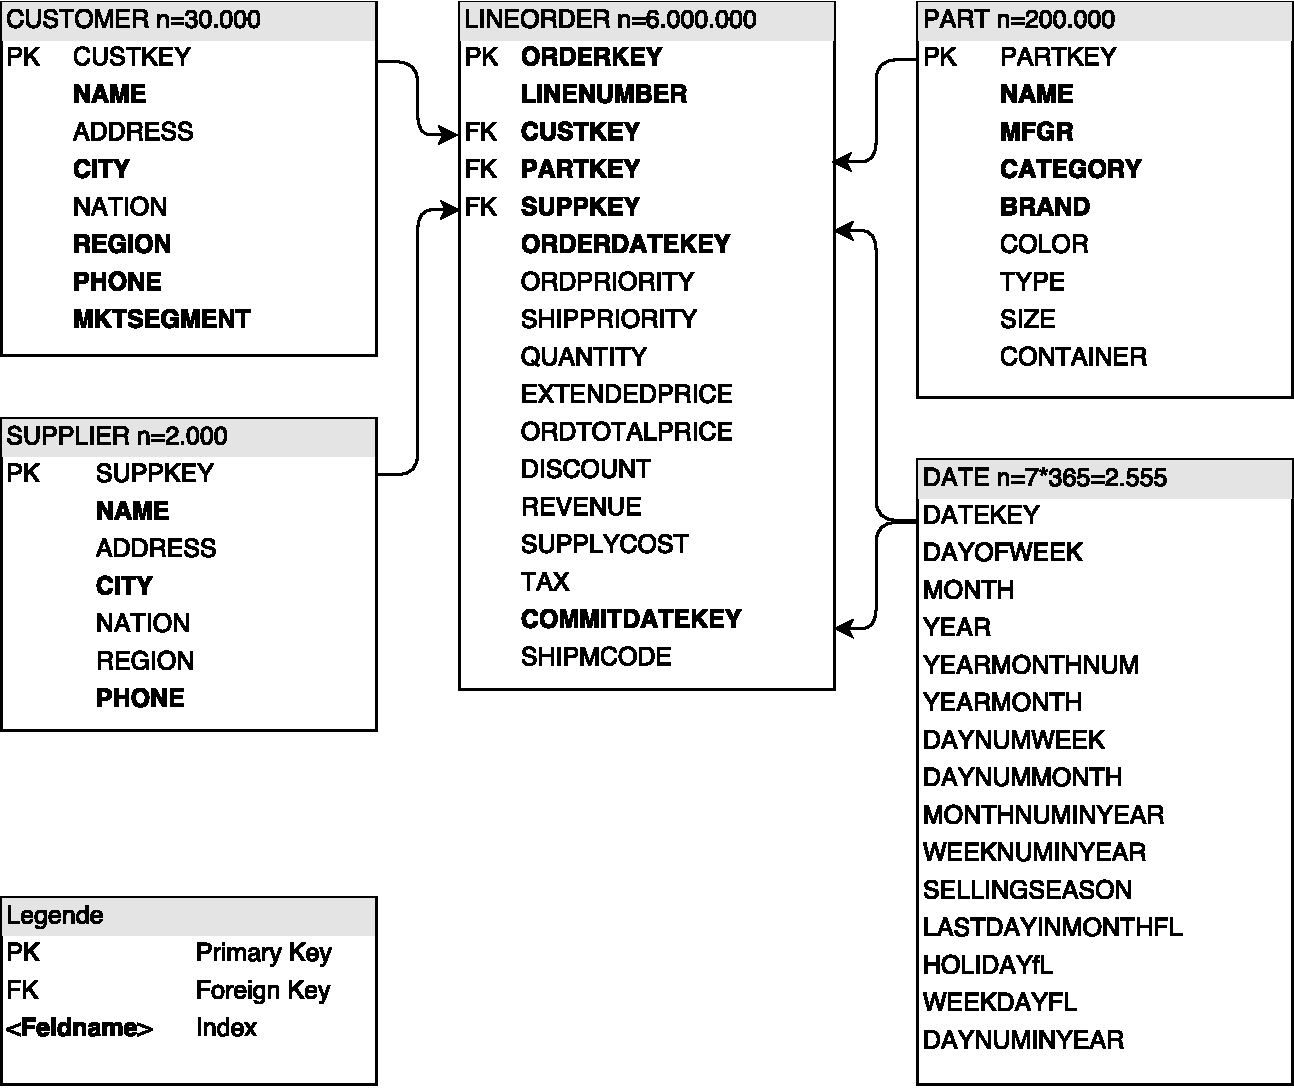
\includegraphics[scale=0.6]{ssbm_basic.pdf}}
%\end{figure}  

Das genutze logische Schema des Benchmarks sieht folgende Tabellen vor: 
\begin{itemize}
	\item \textbf{{\glqq}COSTUMER{\grqq}}: Die Tabelle {\glqq}COSTUMER{\grqq} hat den Primärschlüssel {\glqq}CUSTKEY{\grqq} und umfasst 30 Tausend Datensätze. Indizes werden über die Felder {\glqq}NAME{\grqq}, {\glqq}CITY{\grqq}, {\glqq}REGION{\grqq}, {\glqq}PHONE{\grqq} und {\glqq}MKTSEGMENT{\grqq} gebildet. 
	\item \textbf{{\glqq}PART{\grqq}}: Die Tabelle {\glqq}PART{\grqq} enthält 200 Tausend Datensätze und hat den Primärschlüssel {\glqq}PARTKEY{\grqq}. Indizes werden über die Felder {\glqq}NAME{\grqq}, {\glqq}MFGR{\grqq}, {\glqq}CATEGORY{\grqq} und {\glqq}BRAND{\grqq} gebildet. 
	\item \textbf{{\glqq}SUPPLIER{\grqq}}: Die Tabelle {\glqq}SUPPLIER{\grqq} umfasst 2 Tausend Datensätze und hat den Primärschlüssel {\glqq}SUPPKEY{\grqq}. Indizes werden über die Felder {\glqq}NAME{\grqq}, {\glqq}CITY{\grqq} und {\glqq}PHONE{\grqq} gebildet. 
	\item \textbf{{\glqq}DATE{\grqq}}: Die Tabelle {\glqq}DATE{\grqq} hat den Primärschlüssel {\glqq}DATEKEY{\grqq} und hält 2,555 Tausend Einträge. Ihre Datensätze werden über {\glqq}ORDERDATEKEY{\grqq} und {\glqq}COMMITDATEKEY{\grqq} zugleich aggregiert. 
	\item \textbf{{\glqq}LINEORDER{\grqq}}: Die Tabelle {\glqq}LINEORDER{\grqq} hat den Primärschlüssel {\glqq}ORDERKEY{\grqq} und verweist über die Fremdschlüssel {\glqq}CUSTKEY{\grqq}, {\glqq}PARTKEY{\grqq}, {\glqq}ORDERDATEKEY{\grqq}, {\glqq}COMMITDATEKEY{\grqq} und {\glqq}SUPPKEY{\grqq} auf Datensätze der anderen Tabellen. Die Tabelle umfasst 6 Millionen Einträge. Indizes werden über die Felder {\glqq}ORDERKEY, {\glqq}LINENUMBER, {\glqq}CUSTKEY{\grqq}, {\glqq}PARTKEY{\grqq}, {\glqq}SUPPKEY{\grqq}, {\glqq}ORDERDATEKEY{\grqq} und {\glqq}COMMITDATEKEY{\grqq} gebildet. 
\end{itemize}







